\section{Task and System Framework}
\label{sec:tasks}

\subsection{Analytical task and design requirement}

To better understand the analytical needs of Tree Evolution, we consulted researchers from multiple domains in which tree-structured processes naturally arise and evolve over time. These domains include large language model (LLM) reasoning and agent systems, where researchers are interested in how reasoning structures expand, branch, backtrack, or reorganize across inference steps; database query optimization, where query plans are progressively rewritten into final forms; and program analysis and software engineering, where code revisions can be reflected as structural changes in abstract syntax trees (ASTs). Although these domains have different detailed requirement , they share a common need to analyze how tree structures evolve step by step, how local edits affect the overall topology, and how long evolution processes can be transformed into interpretable patterns.

%Summarized 

From these discussions, we have identified three common analytical tasks.

\textbf{T1. Adjacent-tree comparison.}
A primary need across domains is to compare two consecutive trees as the basic unit of evolution analysis. Analysts want to understand where changes occur in the hierarchy and what kinds of changes they represent, such as node insertion, deletion, attribute update, local restructuring, or subtree replacement. This task is essential because adjacent comparison provides the most direct evidence of the transformation logic between two neighboring states.

\textbf{T2. Cross-step tracing.}
Beyond pairwise comparison, analysts need to follow how a node, subtree, or structurally related region evolves across multiple steps. In particular, they want to track whether a node appears, disappears, changes attributes, or shifts its topological position as the process unfolds. Such tracing is important for understanding propagation effects, repeated revisions, rollback behaviors, and the temporal development of critical structures.

\textbf{T3. Long-sequence simplification.}
When a tree evolves over many steps, analysts need an overview that reveals the global progression of the process. They are interested in identifying salient intervals, key transition points, repeated editing behaviors, and recurring structural patterns, while still being able to relate these summaries back to detailed local changes. Effective summarization is particularly important when critical edits are sparse relative to the full sequence length.

%Based on these tasks, we formulate the following design requirements for a visual analytics system for Tree Evolution.

These analytical tasks suggest that an effective Tree Evolution analysis system should support not only local comparison between adjacent trees, but also the tracing of important structures over time and the summarization of long evolution processes. Accordingly, we derive the following design requirements.

%\textbf{R1. Configurable change modeling.}
%To support \textbf{T1}, the system should allow analysts to define what constitutes change and what remains invariant under different applications and scenarios. Since tree evolution may involve structural edits, attribute updates, or both, the system should provide a flexible way to specify the scope of differencing according to domain needs.
%
%\textbf{R2. Automatic difference detection with context-preserving highlighting.}
%To support \textbf{T1}, the system should automatically detect changes between adjacent trees and visually highlight the corresponding differences. At the same time, the representation should balance cognitive load and fidelity by emphasizing critical changed regions while preserving sufficient unchanged context for interpretation.
%
%\textbf{R3. Cross-step structure tracing.}
%To support \textbf{T2}, the system should automatically trace and present the evolution of analyst-selected nodes or structures across multiple steps. This includes showing appearance, disappearance, attribute changes, and topological relocation, enabling analysts to follow the temporal development of structures of interest.
%
%\textbf{R4. Change intensity indication.}
%To further support \textbf{T2}, the system should quantify and reveal the intensity of structural change over time, so that analysts can quickly identify steps or regions with drastic modifications. Such visual cues help direct attention to critical transitions and potentially abnormal or high-impact changes.
%
%\textbf{R5. Sequence-level overview and trend summarization.}
%To support \textbf{T3}, the system should provide a compact overview of the entire evolution sequence, revealing major trends, salient intervals, and recurring structural patterns. The overview should help analysts move efficiently between macro-level progression understanding and micro-level inspection of specific steps.



\textbf{R1. Flexible difference specification.}
Since different applications may emphasize different forms of change, the system should support flexible specification of what is treated as change and what is treated as invariant, including structural modifications, attribute updates, or both.

\textbf{R2. Context-preserving difference presentation.}
The system should automatically detect and present differences between adjacent trees in a way that emphasizes changed regions while preserving sufficient unchanged context for structural interpretation.

\textbf{R3. Cross-step structure tracing.}
The system should enable analysts to follow the evolution of nodes or substructures across multiple steps, including their emergence, disappearance, attribute variation, and topological relocation.

\textbf{R4. Salient transition identification.}
The system should help analysts identify steps or regions with especially drastic structural changes, providing visual cues that reveal where critical transitions or anomalous edits occur.

\textbf{R5. Sequence-level evolution summarization.}
The system should provide compact overviews of long tree evolution sequences, revealing major trends, salient intervals, and recurring structural patterns while maintaining access to detailed local changes.

\subsection{System framework}

\begin{figure*}
	\centering
	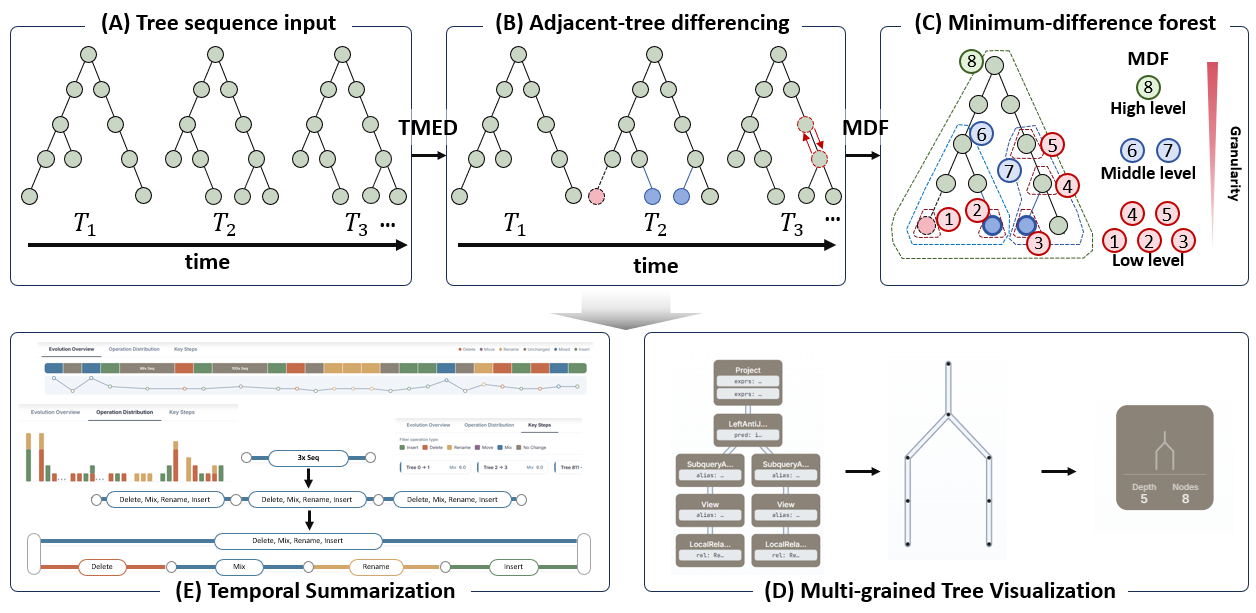
\includegraphics[width=1.95\columnwidth]{figs/framework.png}
	\caption{The workflow of \sysname{}. Need description}
	\label{fig:workflow}
\end{figure*}

To address the above design requirements, we propose a visual analytics framework for exploring the evolution of temporal tree data, as illustrated in Fig.~\ref{fig:workflow}. The framework takes as input a time-ordered sequence of trees \(T_1, T_2, T_3, \dots\), where each tree represents the state of a hierarchical structure at a specific time step. To capture structural evolution, the system first performs adjacent-tree differencing to identify changes between consecutive trees. Specifically, we employ TMED, a tree differencing mechanism that characterizes structural changes in terms of edit operations such as node insertion, deletion, and move/update. Based on the extracted differences, we construct a hierarchical representation termed the minimum-difference forest (MDF), which organizes evolving structures and their changes at multiple levels of granularity. In essence, the MDF serves as an abstraction layer that transforms raw temporal tree sequences into a structured representation suitable for scalable visual analysis.

Built upon the MDF, the framework integrates two coordinated visual components to support the design goals. First, a multi-granularity tree view enables users to inspect structural changes at different levels of detail, thereby supporting both fine-grained change localization (R1) and multi-level exploration from local edits to global patterns (R2). Second, a temporal summary view combines structural change features with temporal information to provide an overview of the evolution process, helping users identify important stages and understand long-term dynamics (R3). By organizing changes hierarchically and presenting them through coordinated views, the framework also reduces visual clutter and improves the scalability of temporal tree analysis (R4). The following sections detail the TMED-based differencing process, the construction of the MDF, and the corresponding visual design and interaction techniques.

